\def\year{2022}\relax
\documentclass[letterpaper]{article}
\usepackage{adjustbox}
 % DO NOT CHANGE THIS
\usepackage{aaai22}  % DO NOT CHANGE THIS
\usepackage{times}  % DO NOT CHANGE THIS
\usepackage{helvet}  % DO NOT CHANGE THIS
\usepackage{courier}  % DO NOT CHANGE THIS
\usepackage[hyphens]{url}  % DO NOT CHANGE THIS
\usepackage{graphicx} % DO NOT CHANGE THIS
\urlstyle{rm} % DO NOT CHANGE THIS
\def\UrlFont{\rm}  % DO NOT CHANGE THIS
\usepackage{natbib}  % DO NOT CHANGE THIS AND DO NOT ADD ANY OPTIONS TO IT
\usepackage{caption} % DO NOT CHANGE THIS AND DO NOT ADD ANY OPTIONS TO IT
\DeclareCaptionStyle{ruled}{labelfont=normalfont,labelsep=colon,strut=off} % DO NOT CHANGE THIS
\frenchspacing  % DO NOT CHANGE THIS
\setlength{\pdfpagewidth}{8.5in}  % DO NOT CHANGE THIS
\setlength{\pdfpageheight}{11in}  % DO NOT CHANGE THIS

\usepackage[ruled,vlined]{algorithm2e}

\usepackage{algorithmic}

\usepackage{amsmath}
\usepackage{bm}
\usepackage{mathrsfs}
\usepackage{amsthm}
\usepackage{amsfonts}
\usepackage{subfigure}
\usepackage{multirow}
\usepackage{url}
\usepackage{array}
\usepackage{amssymb}
\usepackage{booktabs}

\usepackage{color}
\newcommand{\blue}[1]{{{\textcolor{blue}{#1}}}}


\setcounter{secnumdepth}{0} %May be changed to 1 or 2 if section numbers are desired.



\title{A Self-supervised Mixed-curvature Graph Neural Network}
\author{
Li Sun\textsuperscript{\rm 1}\thanks{Corresponding Author: Li Sun, ccesunli@ncepu.edu.cn},  Zhongbao Zhang\textsuperscript{\rm 2}, Junda Ye\textsuperscript{\rm 2}, Hao Peng\textsuperscript{\rm 3}, Jiawei Zhang\textsuperscript{\rm 4}, \\Sen Su\textsuperscript{\rm 2}  and Philip S. Yu\textsuperscript{\rm 5}.
}
\affiliations{
    \textsuperscript{\rm 1}School of Control and Computer Engineering, North China Electric Power University, Beijing 102206, China\\
    \textsuperscript{\rm 2}School of Computer Science, Beijing University of Posts and Telecommunications, China\\
    \textsuperscript{\rm 3}Beijing Advanced Innovation Center for Big Data and Brain Computing, Beihang University, Beijing 100191, China\\
    \textsuperscript{\rm 4}IFM Lab, Department of Computer Science, University of California, Davis, CA, USA\\
    \textsuperscript{\rm 5}Department of Computer Science, University of Illinois at Chicago, IL, USA\\
    ccesunli@ncepu.edu.cn; \{zhongbaozb, susen\}@bupt.edu.cn; penghao@act.buaa.edu.cn; \\jiawei@ifmlab.org; psyu@uic.edu


}
\iffalse
\title{My Publication Title --- Single Author}
\author {
    Author Name
}
\affiliations{
    Affiliation\\
    Affiliation Line 2\\
    name@example.com
}
\fi

\iffalse
\title{My Publication Title --- Multiple Authors}
\author {
    First Author Name,\textsuperscript{\rm 1}
    Second Author Name, \textsuperscript{\rm 2}
    Third Author Name \textsuperscript{\rm 1}
}
\affiliations {
    \textsuperscript{\rm 1} Affiliation 1\\
    \textsuperscript{\rm 2} Affiliation 2\\
    firstAuthor@affiliation1.com, secondAuthor@affilation2.com, thirdAuthor@affiliation1.com
}
\fi


\usepackage{bibentry}

\begin{document}

\maketitle

\begin{abstract}
%Prior works in image conditioned text generation rely on end-to-end training with annotated caption data, which is expensive and computationally intensive.

% chatgpt refined
% Large-scale pre-trained language models (e.g.,GPT) have shown remarkable conversational and reasoning capabilities across many domains. 
% Recent studies has demonstrated the potential of leveraging CLIP latents to extend the capabilities of large language models to vision language tasks(e.g. image captioning) with text-only training. 
% Despite promising results of previous works, there remains a lack of a comprehensive and unified explanation of the prior approaches used and how CLIP latents can be fully leveraged in these applications.

Image captioning aims at generating descriptive and meaningful textual descriptions of images, enabling a broad range of vision-language applications. Prior works have demonstrated that harnessing the power of Contrastive Image Language Pre-training (CLIP) offers a promising approach to achieving zero-shot captioning, eliminating the need for expensive caption annotations. However, the widely observed modality gap in the latent space of CLIP harms the performance of zero-shot captioning by breaking the alignment between paired image-text features. To address this issue, we conduct an analysis on the CLIP latent space which leads to two findings. Firstly, we observe that the CLIP's visual feature of image subregions can achieve closer proximity to the paired caption due to the inherent information loss in text descriptions. In addition, we show that the modality gap between a paired image-text can be empirically modeled as a zero-mean Gaussian distribution. Motivated by the findings, we propose a novel zero-shot image captioning framework with text-only training to reduce the modality gap. In particular, we introduce a subregion feature aggregation to leverage local region information, which produces a compact visual representation for matching text representation. Moreover, we incorporate a noise injection and CLIP reranking strategy to boost captioning performance. We also extend our framework to build a zero-shot VQA pipeline, demonstrating its generality. Through extensive experiments on common captioning and VQA datasets such as MSCOCO, Flickr30k and VQAV2, we show that our method achieves remarkable performance improvements. Code is available at https://github.com/Artanic30/MacCap.

\end{abstract}
\section{Introduction}
From cleaning robots to self-driving cars, autonomous and semi-autonomous agents are becoming increasingly prevalent~\cite{stone2016artificial}. People's understanding of such agents' behaviors can increase their trust in the agents and their ability to collaborate with them~\cite{devin2016implemented,glass2008toward}. An understanding of an agent's behavior could also support people in tasks such as choosing between alternative agents and determining when the agent can be trusted with performing a task autonomously and when the user's attention is needed. For example, if a user can anticipate the behavior of  a self-driving car in different scenarios, she could be more prepared to take control in situations where the car might not perform well on its own.

While prior work has suggested ways to explain individual decisions of an agent to a person~\cite{khan2009minimal,khan2011automatically}, these approaches do not convey a ``global'' view of an agent's policy. Similarly, recent methods for interpretable machine learning~\cite{vellido2012making,doshi2017towards} typically explain a single decision made by a model, e.g. by presenting a simplified model which justifies decisions in a certain region in the space~\cite{ribeiro2016model}. In this paper, we introduce the problem of providing users with a summary of an agent's behavior. This approach aims to provide users with an overview of the agent's global strategy rather than explaining specific decisions  after the fact. 

A trivial way of communicating an agent's behavior is to show past executions or simulations. This approach, however, has important drawbacks. First, many of the situations an agent encounters might be uninteresting to a person (e.g., a self-driving car stuck in traffic for an hour). Second, reviewing long execution traces will require a person to spend a significant amount of time, and people might give up early, or not pay attention, potentially missing important states. Therefore, we seek solutions that extract \emph{effective} summaries which show the actions taken by the agent in key scenarios. Such summaries can reduce the human effort required to review the agent's behavior, while still providing sufficient information about its capabilities. We note that this is analogous to the approach taken in many settings in which people need to assess the performance of other people. For example, sports scouting agencies typically prepare videos that include highlights from players' games to demonstrate their skills\footnote{e.g.,  \url{https://www.youtube.com/watch?v=gX3e0UM-OeM}. We note that while such scouting videos are often biased to showcase only successful actions, we intend that summaries of agent behavior will include states that demonstrates their behavior in different states of interest, whether successful or not.}.  

%The approach of generating summaries that highlight the capabilities of agents is analogous to other settings in which people need to review the performance of other people. For example, sports scouting agencies prepare videos that include highlights from players' games to demonstrate their skills.\footnote{e.g.,  \url{https://www.youtube.com/watch?v=gX3e0UM-OeM}.}

We developed ``HIGHLIGHTS'', an algorithm that extracts important states from an execution trace of an agent in an online manner. Intuitively, a state is important if different actions in that states can lead to substantially different outcomes for the agent. For example, deciding which turn to take when driving in a city will not be considered important if taking the next turn will result in a similar arrival time; deciding whether to exit a highway will be considered more important, as missing the exit can result in a significant delay. Our approach assumes that HIGHLIGHTS has access to the agent's strategy which is described using a  Markov Decision Process (MDP) policy, and quantifies the importance of states based on the agent's Q-values. To provide more context to the user, rather than showing important states in isolation, the algorithm extracts a trajectory that includes neighboring states and composes a summary of the agent's behavior from these trajectories.

We used HIGHLIGHTS to create summaries of agents playing Mrs. Pacman~\cite{rohlfshagen2011ms} and evaluated these summaries in a human-subject experiment. We compared HIGHLIGHTS summaries with two baselines. One baseline generated summaries by extracting random trajectories of the agent, which will, on average, include states that are more likely to be encountered. The other baseline generated summaries by extracting the first trajectories the agent encountered, which is akin to having a user watch the agent until she runs out of time. In the experiment, participants were shown summaries of different Pacman agents which varied in their performance, and were asked to select an agent to play on their behalf.  They were also asked to rate the helpfulness of different summaries for evaluating an agent's capabilities. 
%They were also shown pairs of summaries of the \emph{same} Pacman agent and were asked to subjectively assess how helpful each of the summaries is for understanding that agent's capabilities. 
Our results show that HIGHLIGHTS led to improved objective performance of participants: they were significantly more likely to choose the better performing agent when the HIGHLIGHTS summaries were shown. HIGHLIGHTS summaries were also rated as more helpful by the study participants. 

%can be condensed to two sentences if needed
One limitation of the HIGHLIGHTS algorithm is that it does not consider the diversity of states in the summary, and therefore if important states are similar to each other, the summary will consist of similar trajectories, thus conveying less new information to users. To mitigate this problem, we developed a variant of the HIGHLIGHTS algorithm which, in addition to state importance, takes into consideration the similarity of the state to other states in the summary. This extension further improved participants' ability to assess the performance of different agents.

The contributions of the paper are threefold: (1) we introduce and formalize the problem of summarizing an agent's behavior to people; (2) we develop HIGHLIGHTS and HIGHLIGHTS-DIV, algorithms that automatically extract summaries of an agent's policy, and (3) we conduct human-subject experiments, showing that summaries generated by HIGHLIGHTS and HIGHLIGHTS-DIV were preferred by participants and improved their ability to assess the capabilities of agents compared to the baseline summaries.

%!TEX root = ./SelfMGNN.tex

\section{Preliminaries and Problem Definition}

% Prior to introducing the studied problem and proposed approach, we provide some important preliminaries in this section. 
% Throughout the paper, 
% we denote the Euclidean norm and inner product by $\| \cdot \|_2$ and $\langle \cdot, \cdot \rangle$, respectively.
In this section, we first present the preliminaries and notations necessary to construct a mixed-curvature space.
%(more details can be found in textbooks [28, 39]), 
%including the Riemannian manifold and constant-curvature space. 
Then, we formulate the problem of \emph{self-supervised graph representation learning in the mixed-curvature space}.


\subsection{Riemannian Manifold}

A smooth \emph{manifold} $\mathcal M$ generalizes the notion of the surface to higher dimensions.
Each point $\mathbf x \in \mathcal M$ associates with a \emph{tangent space} $\mathcal T_\mathbf x\mathcal M$, the first order approximation of $\mathcal M$ around $\mathbf x$, which is locally Euclidean.
On tangent space $\mathcal T_\mathbf x\mathcal M$, the \emph{Riemannian metric}, $g_\mathbf x (\cdot, \cdot) : \mathcal T_\mathbf x\mathcal M  \times \mathcal T_\mathbf x\mathcal M \to \mathbb R$, defines an inner product so that geometric notions can be induced.
The tuple $(\mathcal M, g)$ is called a \emph{Riemannian manifold}.

Transforming between the tangent space and the manifold is done via exponential and logarithmic maps, respectively.
For $\mathbf x \in \mathcal M$, 
the  \emph{exponential map} at $\mathbf x$, 
$\mathbf{exp}_\mathbf x(\mathbf v): \mathcal T_\mathbf x\mathcal M \to \mathcal M$, 
projects the vector $\mathbf v \in \mathcal T_\mathbf x\mathcal M$ onto the manifold $\mathcal M$.
The \emph{logarithmic map} at $\mathbf x$, 
$\mathbf{log}_\mathbf x(\mathbf y): \mathcal M \to \mathcal T_\mathbf x\mathcal M$, 
projects the vector $\mathbf y \in \mathcal M$ back to the tangent space $\mathcal T_\mathbf x\mathcal M$.
For further expositions, please refer to mathematical materials \cite{Spivak1979,Hopper2010}.

\subsection{Constant Curvature Space}

The Riemannian metric also defines a curvature at each point $\kappa(\mathbf x)$, 
which determines how the space is curved.
If the curvature is uniformly distributed,  
$(\mathcal M, g)$ is called a \emph{constant curvature space} of curvature $\kappa$. 
There are $3$ canonical types of constant curvature space that we can define with respect to the sign of the curvature: 
a positively curved spherical space $\mathbb S$ with $\kappa>0$, 
a negatively curved hyperbolic space $\mathbb H$ with $\kappa<0$ 
and the flat Euclidean space $\mathbb E$  with $\kappa=0$.

\noindent\textbf{Note that}, $\| \cdot \|_2$ denotes the Euclidean norm in this paper.

\subsection{Problem Definition}
In this paper, we propose to study the self-supervised graph representation learning in the mixed-curvature space.
Without loss of generality,
a graph is described as $G = (V, E, \mathbf X)$, 
where $V = \{v_1,  \cdots, v_n\}$ is the node set and $E =\{ (v_i,  v_j ) | \  v_i,  v_j \in V\}$ is the edge set. 
We summarize the edges in the adjacency matrix $\mathbf G$, where $\mathbf G_{ij}=1$ iff $(v_i,  v_j ) \in E$, otherwise $0$.
Each node $v_i$ is associated with a feature vector $\mathbf x_i \in \mathbb R^d$, and matrix $\mathbf{X} \in \mathbb{R}^{|V| \times d}$ represents the features of all nodes.
Now, we give the studied problem:
\newtheorem*{def1}{Problem Definition (Self-supervised graph representation learning in the mixed-curvature space)} 
\begin{def1}
Given a graph $G = (V, E, \mathbf X)$, 
the problem of self-supervised graph representation learning in the mixed-curvature space
is to learn an encoding function $\Phi: V \to \mathcal P$ that maps the node $v$ to a vector $\boldsymbol z$ in a mixed-curvature space $\mathcal P$ that captures the intrinsic complexity of graph structure without using any label information. 
\end{def1}

In other words, the graph representation model should align with the complex graph structures 
— hierarchical as well as cyclical structure, 
and can be learned without external guidance (labels). 
% The representation space of constant curvature works well on particular kinds of structure that they were designed for. % \cite{HGNN,ZhangWSLS21}.
% Instead of the constant-curvature space, the mixed-curvature space is called in fact to cover the intrinsic complicated structures of the graphs.
Graphs in reality are usually mixed-curvatured rather than structured uniformly, i.e., in some regions hierarchical, while in others cyclical.
A constant-curvature model (e.g., hyperbolic, spherical or the Euclidean model) benefits from their specific bias to better fit particular structure types. 
To bridge this gap, we propose to work with the \textbf{mixed-curvature space} to cover the  complex graph structures in real-world applications.



\section{Methodology}
\label{sec:methodology}
RGB images depict objects based on color differences that match human perception. However, objects with similar colors may not have enough color contrast to show their shape. By contrast, polarized light is strongly linked to the material of objects and the orientation of the reflecting surface, enabling it to reveal material properties that make object boundaries visible even when colors are similar (\textit{e.g.}, Fig. \ref{fig:samples} (a) and (b)). In spite of that, polarization cues may be weak in certain lighting conditions or viewing angles (\textit{e.g.}, Fig. \ref{fig:samples} (c)). Including polarization measurements naively in existing car detection methods may not necessarily yield the expected performance improvement. How to effectively integrate RGB and polarization features is a key challenge to be addressed to achieve robust car detection.

We introduce a novel Polarization Car Detection Network (PCDNet) that is capable of exploring and integrating polarized material cues for robust car detection. As shown in Fig. \ref{fig:pipeline}, PCDNet takes as input the RGB intensity, trichromatic AoLP and DoLP, and outputs car detections. The AoLP and DoLP are first integrated into a comprehensive and semantically meaningful polarization feature representation by a Polarization Integration (PI) module for the ease of the following feature extraction and fusion. Then, the RGB and polarization features are separately fed into two branches of CSPDarkNet \cite{wang2020cspnet} encoder, each consisting of five stages to extract multi-level contextual features. The Material Perception (MP) module, which aims to extract the intrinsic material properties of cars across the whole learning samples, is applied to different levels of extracted features. The MP module has a specific design for low-level features (MSP with spatial specialization) and high-level features (MCP with channel specialization), respectively. For multimodal feature fusion, the Cross-Domain Demand Query (CDDQ) module assigns fusion weights adaptively and conducts dynamic fusion in a request-and-complement manner. Finally, based on the fused features, we adopt the anchor-based detection head from YOLOv7 \cite{wang2022yolov7} to generate final classifications and bounding boxes.

\subsection{Polarization Integration (PI)}
AoLP $\phi$ and DoLP $\rho$ reveal object/scene materials from two different aspects. Polarization Integration (PI) module is designed to combine them into an unified and semantically meaningful polarization representation $F_{pol}$ for the ease of the following feature extraction and fusion. As the captured polarization angle is more likely random at regions with a low polarization degree, PI filters the AoLP measurement based on the DoLP. In addition, PI also extracts and integrates the edge information in DoLP measurement to help the distinction of objects with different materials. Formally,
\begin{align} \label{eq:pim}
    F_{pol} &=\vartheta_{3\cdot 1}([\vartheta_{3\cdot 1}(F_{\phi\rho}), \vartheta_{3\cdot 1}(\rho+\mathbb{E}(\rho))]), \\
    F_{\phi\rho} &=\phi\otimes(\vartheta_{3\cdot 1}([\hat{\mathbb{A}}(\rho),\hat{\mathbb{M}}(\rho)])+\sigma(\mathbb{M}(\vartheta_{3\cdot 1}(\rho)))),
\end{align}
where $\vartheta_{k\cdot s}$ denotes a $k \times k$ convolution with a stride of $s$, followed by a batch normalization and a SiLU activation function. $[\cdot]$ indicates the concatenation operation over the channel dimension. $\mathbb{E}$ refers to the Scharr edge extractor. $\otimes$ is the element-wise multiplication. $\hat{\mathbb{A}}$ and $\hat{\mathbb{M}}$ are the average and max pooling in the channel dimension, respectively. $\mathbb{M}$ is the max pooling in the spatial dimension with a kernel size of 5. And $\sigma$ is the Sigmoid activation.

\subsection{Material Perception (MP)}
Despite the cars in different scenarios may have diverse visual appearances such as different colors and textures, they are typically share similar materials including glass, rubber, metal, etc. Fortunately, polarization can robustly reveal the intrinsic physical properties of these materials. Inspired by this, we design the Material Perception (MP) strategy to explore
% and memorize 
the discriminative and invariant material features of cars across different scenarios. Considering the different characteristics of different levels of features, \textit{i.e.}, low-level features have larger spatial sizes and keep rich and detailed low-level information while high-level features contain more semantic cues distributed in more feature channels, MP is instantialized as Material Spatial/Channel Perception (MSP/MCP) modules for the low-/high-level polarization features, respectively. Formally, MSP/MCP can be described as:
\begin{align} \label{eq:mpm}
    MSP(F) &=\varrho_{2\cdot2}(\varrho_{2\cdot2}(\vartheta_{3\cdot2}(\vartheta_{3\cdot2}(F)))), \\
    MCP(F) &=\varrho_{2\cdot2}(\mathcal{M}((\vartheta_{1\cdot1}(\vartheta_{3\cdot2}(F))))), \\
    \mathcal{M}(x) &=x+x\otimes\sigma(m_2(m_1(\bar{\mathbb{A}}(x)))),
\end{align}
where $\varrho_{k\cdot s}$ denotes a $k \times k$ transposed convolution with a stride of $s$, followed by a batch normalization and a SiLU activation function. $\mathcal{M}(\cdot)$ is the perception scheme with two independent perception matrices in fully connected layers named $m_1$ and $m_2$. And $\bar{\mathbb{A}}$ is global average pooling.

\subsection{Cross Domain Demand Query (CDDQ)}
Polarization and RGB features are different types of representations of the scenes and simply combing them may dilute the useful clues of the cars originally presented in the individual modality or amplify the background interference. We address this issue by introducing the Cross-Domain Demand Query (CDDQ) module for effective multimodal feature fusion, taking into account both the context and quality of each modality feature. CDDQ takes as input the RGB features $F_{rgb}$ and polarization representations $F'_{pol}$. It first utilizes a Spatial Demand Map Delivery (SDMD) block to generate enhanced RGB features $F_{rgb}^{*}$ and distill informative and required polarization features $F_{pol}^{*}$ and then obtains fused features $F_{fused}$ through a Channel Weight Dynamic Assignment (CWDA) block:
\allowdisplaybreaks\begin{align}
    F_{rgb}^{*} &=F_{rgb}+F''_{rgb} = F_{rgb}+\mu\otimes F'_{rgb} \nonumber \\
        &=F_{rgb}+\mu\otimes \eta\otimes F_{rgb}, \\
    \eta &=\sigma(\vartheta_{1\cdot1}(\bar{\mathbb{M}}(F_{rgb}))+\vartheta_{1\cdot1}(\bar{\mathbb{A}}(F_{rgb}))), \\
% \end{align} 
% \begin{align}
    \mu &=\sigma(\vartheta_{7\cdot1}([\hat{\mathbb{A}}(F'_{rgb}), \hat{\mathbb{M}}(F'_{rgb})])), \\
    F_{pol}^{*} &=F'_{pol}+\vartheta_{3\cdot1}(\mathbb{A}(\mu))\otimes F'_{pol}, \\
    F_{fused} &=\vartheta_{1\cdot1}([\alpha\times F_{rgb}^{*},\beta\times F_{pol}^{*}]), \\
    \alpha, \beta &=\delta(\langle\sigma(fc(si(fc([\bar{\mathbb{A}}(F_{rgb}^{*}), \bar{\mathbb{A}}(F_{pol}^{*})]))))\rangle),
\end{align}
where $\eta$ is the channel attention vector. $\mu$ is the spatial attention map which also serves as the guidance of the informative polarization cues request process. $\mathbb{A}$ is an average pooling with a kernel size of 3. $\bar{\mathbb{M}}$/$\bar{\mathbb{A}}$ denotes global max/average pooling. $\alpha$ and $\beta$ are dynamic fusion weights assigned to the RGB and polarization features, respectively, with a constraint of being non-negative and summing up to 1 for each channel position. $fc$ is the fully connected layer and $\langle\cdot\rangle$ is the split operation over the channel dimension. $si$ and $\delta$ are the SiLU and Softmax activation functions, respectively.

\begin{figure}[ht]
    \begin{center}
        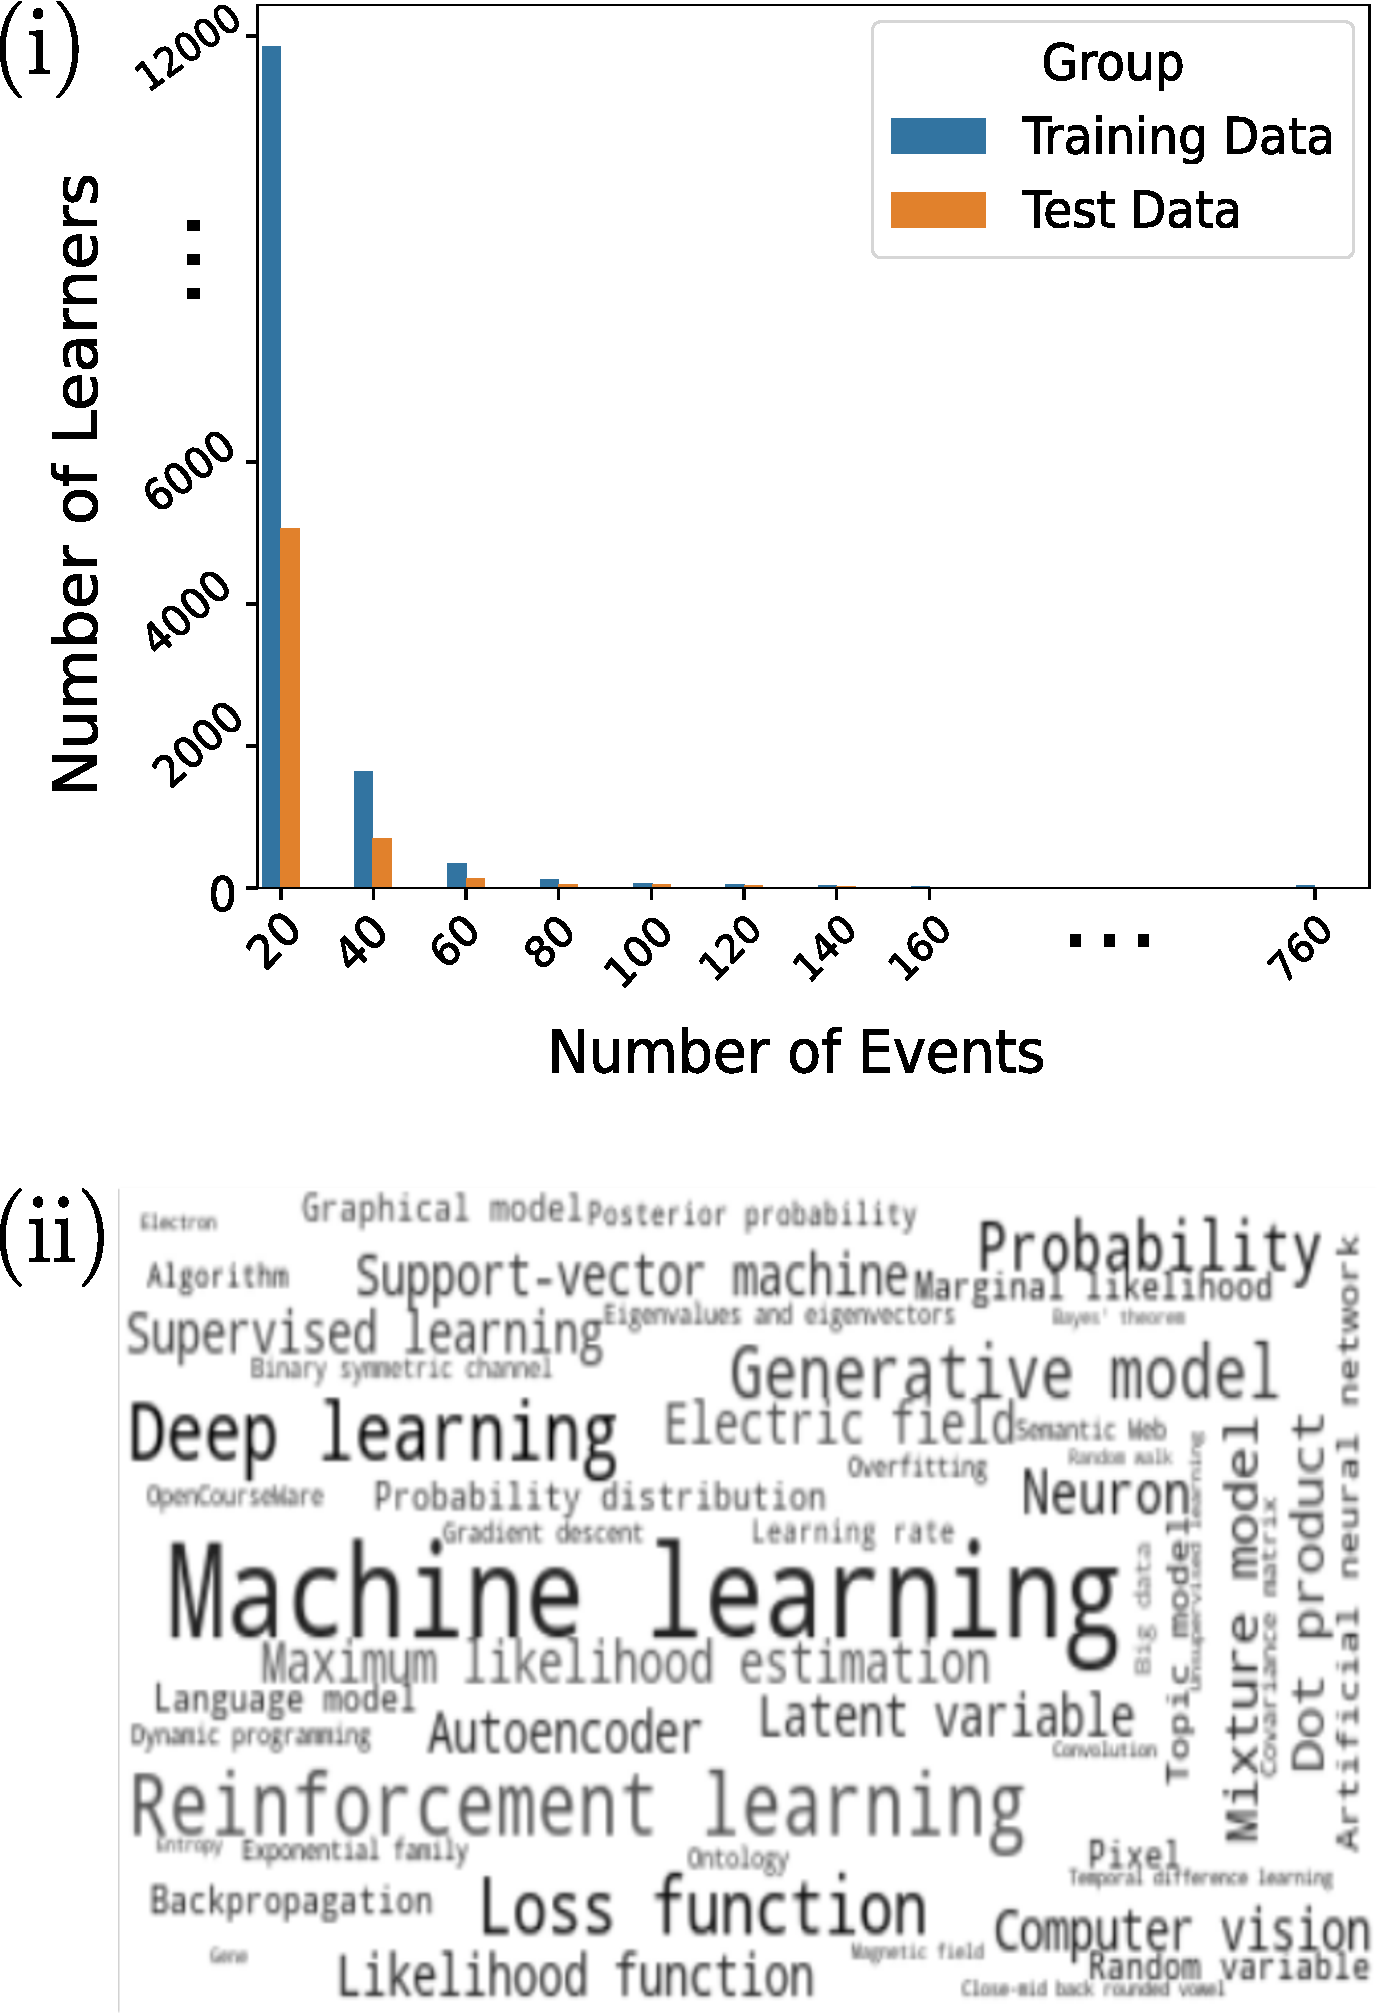
\includegraphics[width=1\linewidth]{figure/dataset.pdf}
    \end{center}
    \caption{
    RGBP-Car Examples. The first column displays the RGB intensity (top) and the corresponding annotation (bottom). The next three columns show the AoLP (top) and DoLP (bottom) measurements for the red, green, and blue channels, respectively. From top to bottom are scenes of stopped cars in a rainy parking lot, dense cars in an outdoor parking lot, and driving cars on a clear night road, respectively. 
    (The low-light RGB image is enhanced by ZeroDCE \cite{guo2020zero} (with \orange{orange} frame) for visualization.)}
    \label{fig:samples}
\end{figure}


\section{Experiments}
\label{sec:experiment}

\begin{table}[t]
\centering
\small
\resizebox{0.99\linewidth}{!}{
\begin{tabular}{lcccc}
\multirow{2}{1.5cm}{\textbf{Methods}} & \multicolumn{2}{c}{\textbf{Far-OOD}} & \multicolumn{2}{c}{\textbf{Near-OOD}}\\
\cmidrule{2-5}
& \textbf{FPR95}  & \textbf{AUROC} & \textbf{FPR95}  & \textbf{AUROC}\\
& $\downarrow$ & $\uparrow$ & $\downarrow$ & $\uparrow$ \\
\toprule
\emph{Using model outputs}\\
MSP~\cite{hendrycks2016baseline} & 52.11 & 91.79 & 64.66 & 85.28 \\
ODIN~\cite{liang2018enhancing}  & 26.47 & 94.48 & 52.32 & 88.90\\
GODIN~\cite{hsu2020generalized}  & 17.42  & 95.84 & 60.69 & 82.37 \\
Energy score~\cite{liu2020energy}  & 28.40 & 94.22 & 50.64 & 88.66 \\
ReAct~\cite{sun2021react} & 33.12 & 94.32 & 53.51 & 88.96\\
GradNorm~\cite{huang2021importance} & 24.79 & 92.58 & 65.44 & 79.31\\
LogitNorm~\cite{wei2022mitigating}  & 19.61 & 95.51 & 55.08 & 88.03\\
DICE~\cite{sun2022dice}  & 20.83 & 95.24 & 58.60 & 87.11 \\
\midrule
\emph{Using feature representations}\\
Mahalanobis~\cite{lee2018simple} & 44.55 & 82.56 & 87.71 & 78.93 \\
KNN~\cite{sun2022knn}  & 18.50 & 96.36 & 58.34 & 87.90 \\
\midrule 
 \name (ours) & \textbf{14.99} & \textbf{97.15}  & \textbf{50.10} &  \textbf{89.80}\\
 & $\pm{0.87}$ & $\pm{0.27}$ & $\pm{1.09}$ & $\pm{0.65}$\\
\bottomrule
\end{tabular}}
\caption{\small Performance comparison on near-OOD and far-OOD detection task. Architecture used is DenseNet-101 and ID data is CIFAR-10. We report the mean and variance across 3 training runs.}
\label{tab:hard_ood}
\end{table}
\begin{table}[t]
\small
\centering
\resizebox{0.99\linewidth}{!}{
\begin{tabular}{lccc}
\textbf{Method} & \textbf{FPR95}  & \textbf{AUROC} & \textbf{ID Acc.}\\
& $\downarrow$ & $\uparrow$ & $\uparrow$ \\
\toprule
\emph{Methods using model outputs}\\
MSP~\cite{hendrycks2016baseline} & 77.59 & 76.47 &  75.14\\
ODIN~\cite{liang2018enhancing} & 56.39 & 86.02 & 75.14\\
GODIN~\cite{hsu2020generalized} & 44.08 &  89.05 & 74.37\\
Energy score~\cite{liu2020energy} & 57.07 &  84.83 &  75.14\\
ReAct~\cite{sun2021react} & 75.06 & 79.51 & 66.56\\
GradNorm~\cite{huang2021importance} & 63.05 & 79.80 & 75.14\\
LogitNorm~\cite{wei2022mitigating} & 61.10 & 84.72 & 75.42\\
DICE~\cite{sun2022dice} & 49.72 & 87.23 & 68.65 \\
\midrule 
\emph{Methods using feature representations}\\
Mahalanobis~\cite{lee2018simple} & 56.93 & 80.27 &  75.14\\
KNN~\cite{sun2022knn} & 47.21 & 85.27 & 75.14\\
\midrule 
 \name (ours) & \textbf{31.25} & \textbf{90.76} & \textbf{75.59}\\
& $\pm{1.25}$ & $\pm{0.36}$ & $\pm{0.08}$\\
\bottomrule
\end{tabular}}
\caption{\small Performance comparison on CIFAR-100 dataset. We use DenseNet-101 for all baselines. Best  results are in \textbf{bold}. We report the mean and variance across 3 different training runs.}
\label{tab:cifar-100}
\end{table}
In this section, we extensively evaluate the effectiveness of our proposed method. 
The goal of our experimental sections is to mainly answer the following questions: (1) Can \name alleviate the curse of dimensionality? (2) How does \name compare against the state-of-the-art OOD detection methods?  Due to space constraints, extensive experimental details are in Appendix C. Our code is open-sourced for the research community.


\subsection{Evaluation on Common Benchmarks}
\label{subsec:common_benchmark}

\noindent \textbf{Datasets.} In this section, we make use of commonly studied CIFAR-10 (10 classes) and CIFAR-100 (100 classes)~\cite{krizhevsky2009learning} datasets as ID. Both datasets consist of images of size $32 \times 32$. We use the standard split with $50,000$ images for training and $10,000$ images for testing. We evaluate the methods on common OOD datasets: \texttt{Textures}~\cite{cimpoi2014describing}, \texttt{SVHN}~\cite{svhn}, \texttt{LSUN-Crop}~\cite{yu2015lsun}, \texttt{LSUN-Resize}~\cite{yu2015lsun}, \texttt{iSUN}~\cite{xu2015turkergaze}, and \texttt{Places365}~\cite{zhou2017places}. Images in all these test datasets are of size $32 \times 32$. 


\paragraph{Evaluation metrics.} We compare the performance of various methods using the following metrics: 
(1) {FPR95} measures the false positive rate (FPR) of OOD samples when $95\%$ of ID samples are correctly classified;
(2) {AUROC} is the area under the Receiver Operating Characteristic curve; 
and (3) {ID Acc.} measures the ID classification accuracy.

\vspace{0.2cm}
\noindent \textbf{Comparison with competitive methods.} In Table~\ref{tab:cifar-100}, we provide a comprehensive comparison with competitive OOD detection baselines on  CIFAR-100. {We provide a detailed description of baseline approaches in Appendix C.3.} We observe that our proposed method \name significantly outperforms the latest rivals. For a fair comparison, we divide the baselines into two categories: methods using model outputs and methods using feature representations.
From Table~\ref{tab:cifar-100}, we highlight two salient observations: (1) Considering methods based on feature representations, \name outperforms KNN (non-parametric) and Mahalanobis (parametric) by \textbf{15.96\%} and \textbf{25.68\%} respectively in terms on FPR95. The results validate that learning feature subspace effectively alleviates the ``curse-of-dimensionality" problem that is troubling the existing KNN approach. (2) Further, \name also performs better than output-based methods such as ReAct~\cite{sun2021react}. Specifically, with CIFAR-100 as ID, \name provides a $\mathbf{43.81}\%$ improvement in FPR95 as compared to ReAct~\cite{sun2021react}. Notably, \name provides a \textbf{18.47\%} improvement compared to~\cite{sun2022dice}, a post-hoc sparsification method. While DICE can severely affect the ID test accuracy (68.65\%), \name exhibits stronger classification performance (75.59\%) by baking in the inductive bias of subspaces through training. An extensive discussion is provided in Section~\ref{sec:discussion}. 



\paragraph{Evaluation on near-OOD data.} In Table~\ref{tab:hard_ood}, we compare the performance in detecting near-OOD data, which refers to samples near the ID data. Near-OOD is particularly challenging to detect, and can often be misclassified as ID. We report the performance on CIFAR-10 (ID) vs. CIFAR-100 (OOD), which is the most commonly used dataset pair for this task. We observe that \name consistently outperforms existing algorithms for near-OOD detection tasks, further demonstrating its strengths. Compared to KNN, \name reduces the FPR95 by 8.24\%. For completeness, we also provide far-OOD evaluation results on CIFAR-10, where \name achieves an average FPR95 of 14.99\%. Full result on each test dataset for CIFAR-10 is available in Appendix D.4.



\begin{table}[t]
\small
\centering
\resizebox{0.95\linewidth}{!}{
\begin{tabular}{lccc}
\textbf{Method} & \textbf{Dataset (ID)} & \textbf{FPR95}  & \textbf{AUROC} \\
& & $\downarrow$ & $\uparrow$  \\
\toprule
Mahalanobis~\cite{lee2018simple} & CIFAR-10 & 44.55 & 82.56  \\

\name (w. Mahalanobis) & CIFAR-10 &  \textbf{34.68} &  \textbf{87.87} \\
\midrule
Mahalanobis~\cite{lee2018simple} & CIFAR-100 & 56.93 & 80.27  \\

\name (w. Mahalanobis) & CIFAR-100 &  \textbf{55.05} &  \textbf{80.77} \\
\bottomrule
\end{tabular}}
\caption{\small \name is also compatible with parametric approaches such as Mahalanobis distance~\cite{lee2018simple}. The model is DenseNet. All values are averaged over six OOD test datasets.}
\label{tab:compatibility}
\end{table}


\paragraph{Compatibility with other distance-based approaches.} 

Beyond KNN~\cite{sun2022knn}, the Mahalanobis distances~\cite{lee2018simple} is also one of the most popular distance-based approaches to detect OOD. 
However, all prior solutions measure the distance with a full feature space which can also suffer from the curse of dimensionality. 
In this section, we show that subspace learning can also benefit parametric approaches like Mahalanobis distance~\cite{lee2018simple}. In Table~\ref{tab:compatibility}, we compare the OOD detection performance of using Mahalanobis distance on the vanilla model and the model trained with \name. 
We see that coupling subspace learning (in training) with Mahalanobis distance (in testing) reduces FPR95 by {9.87\%} and {1.88\%} on CIFAR-10 and CIFAR-100 datasets respectively.

\begin{table}[t]
\small
\centering
\resizebox{0.55\linewidth}{!}{
\begin{tabular}{lcc}
\toprule
\multirow{2}{2cm}{\textbf{Training Method}} &  CIFAR-10 & CIFAR-100 \\ 
& \multicolumn{2}{c}{(Train time in hours)} \\
\midrule
Standard & $2.10$ & $2.25$\\ 
 \name & $1.75$ & $1.89$ \\
\bottomrule
\end{tabular}}
\caption{\small \textbf{Computational cost for training}. trained using ResNet-101. 
Model used is DenseNet-101. For the comparison, we used the software configuration as reported in Appendix C.2.}
\label{tab:train_time}
\end{table}
% 
\paragraph{Computational complexity.}  In Table~\ref{tab:train_time}, we compare the training time of \name with the standard training method using cross-entropy loss. We observe that training using \name incurs no additional computation overhead but rather is slightly more efficient compared to standard training procedures. This is because we perform gradient descent only on a subset of weights corresponding to the selected feature subspace. Thus, our method overall leads to faster updates and convergence. {In Appendix D.1, we further show that
\name remains competitive and outperforms the KNN counterpart on other common architecture.}
\section{Related Work}
In this section, we briefly review some existing neural matching models and graph neural networks.

\subsection{Neural Matching Models}
Most neural matching models fall within two categories: representation-focused models, e.g. DSSM \cite{huang2013learning}, ARC-I \cite{hu2014convolutional}, CDSSM \cite{shen2014latent}, and interaction-focused models, e.g. MatchPyramid \cite{pang2016text}, DRMM \cite{guo2016deep}, PACRR \cite{hui2017pacrr}, KNRM \cite{xiong2017end}.

The representation-focused models follow the representation learning approach adopted in many natural language processing tasks. Queries and documents are projected into the same semantic space individually. The cosine similarity is then used between their high-level text representations to produce the final relevance score. For example, DSSM \cite{huang2013learning}, one of the earliest neural relevance matching models, employs simple dense neural layers to learn high-level representations for queries and documents. To enhance the projecting function, ARC-I \cite{hu2014convolutional} and CDSSM \cite{shen2014latent} devoted much effort into convolutional layers later on. 

In comparison, interaction-focused methods model the two text sequences jointly, by directly exploiting detailed query-document interaction signals rather than high-level representations of individual texts. For example, DRMM \cite{guo2016deep} maps the local query-document interaction signals into a fixed-length histogram, and dense neural layers are followed to produce final ranking scores. \citet{xiong2017end} and \citet{dai2018convolutional} both use kernel pooling to extract multi-level soft match features. Many other works rely on convolutional layers or spatial GRU over interaction signals to extract ranking features  
such as \cite{pang2016text,pang2017deeprank,hui2017pacrr,hui2018co,fan2018modeling}, which considers just local word connections. 

There are also several studies investigating how to apply BERT in ranking, e.g.  \citet{dai2019deeper} and \citet{macavaney2019cedr}. A common approach is to concatenate the document and query text together and feed them into the next sentence prediction task, where the `[CLS]' token embeds the representation of the query-document pair. 
\begin{figure*}[h]
	\centering
	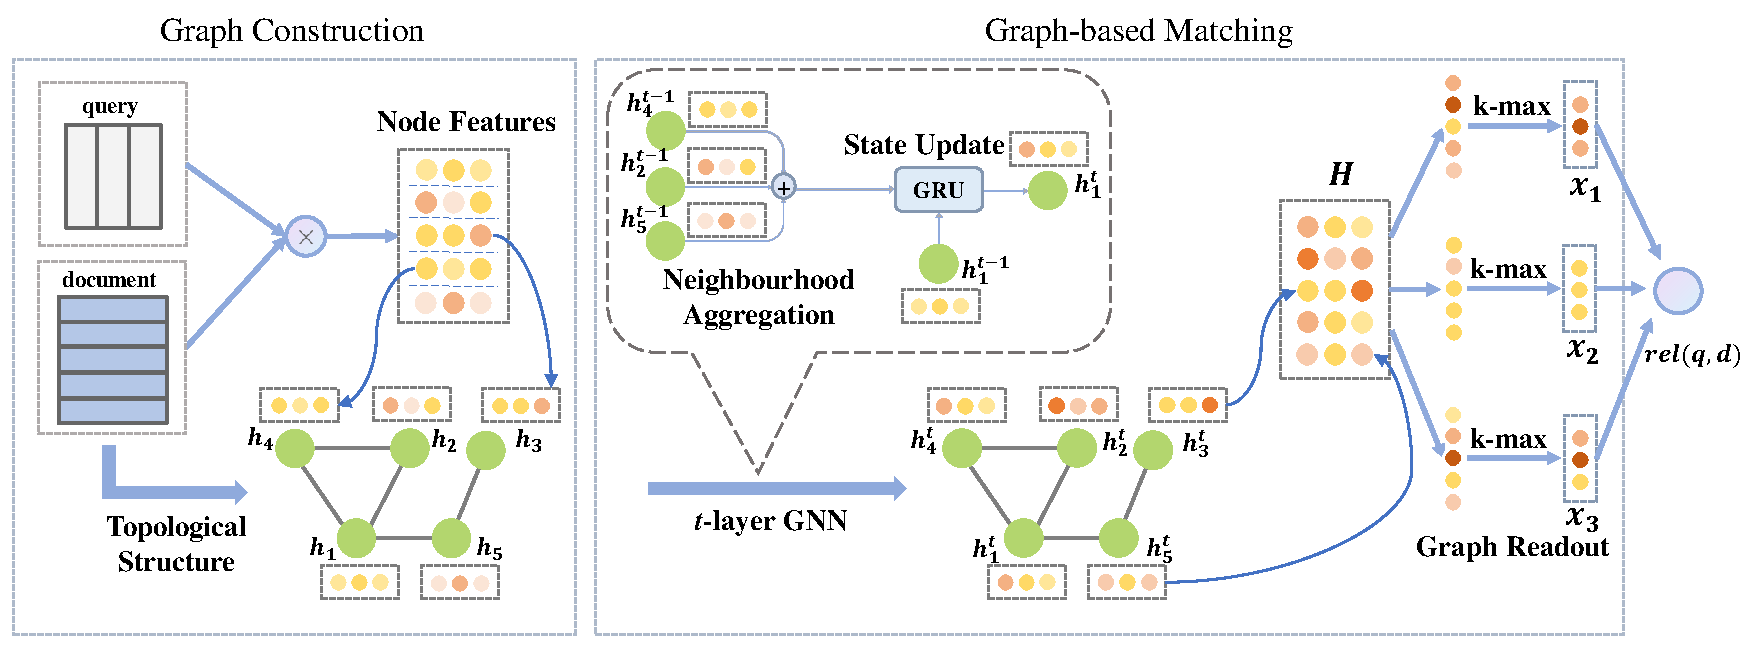
\includegraphics[width=\textwidth]{./pics/grmm.pdf}
	\caption{The workflow of the GRMM model. The document is first transformed into the graph-of-word form, where the node feature is the similarity between the word and each query term. Then, graph neural networks are applied to propagate these matching signals on the document graph. Finally, to estimate a relevance score, top-$k$ signals of each query term are chosen to filter out irrelevant noisy information, and their features are fed into a dense neural layer. }
	\label{fig:2} 
\end{figure*}

Nevertheless, the majority of existing neural matching models only take the linear text sequence, inevitably limiting the model capability. To this end, we propose to break the linear text format and represent the document in a flexible graph structure, where comprehensive interactions can be explicitly modeled. 



\subsection{Graph Neural Networks}
Graph is a kind of data structure which cooperates with a set of objects (nodes) and their relationships (edges). Recently, researches of analysing graphs with machine learning have attracted much attention because of its great representative power in many fields. 

Graph neural networks (GNNs) are deep learning based methods that operate in the graph domain. The concept of GNNs is previously proposed by  \cite{scarselli2008graph}. Generally, nodes in GNNs update own hidden states by aggregating neighbourhood information and mixing things up into a new context-aware state. There are also many variants of GNNs with various kinds of aggregators and updaters, such as \cite{li2016gated,kipf2017semi,hamilton2017inductive,velivckovic2018graph}. 

Due to the convincing performance and high interpretability, GNNs have become a widely applied structural analysis tool. Recently, there are many applications covering from recommendation \cite{wu2019session,li2019fi} to NLP area, including text classification \cite{yao2019graph,zhang2020every}, question answering \cite{de2019question}, and spam review detection \cite{li2019spam}.

In this work, we employ GNNs in the relevance matching task to extract implicit matching patterns from the query-document interaction signals, which is intrinsically difficult to be revealed by existing methods. 



\section{Acknowledgments}
Hao Peng is partially supported by the National Key R\&D Program of China through grant 2021YFB1714800,  NSFC through grant 62002007, S\&T Program of Hebei through grant 21340301D.
Sen Su and Zhongbao Zhang are partially supported by the National Key Research and Development Program of China under Grant 2018YFB1003804, NSFC under Grant U1936103 and 61921003.
Philip S. Yu is partially supported by NSF under grants III-1763325, III-1909323,  III-2106758, and SaTC-1930941.
Jiawei Zhang is partially supported by NSF through grants IIS-1763365, IIS-2106972 and by UC Davis.
This work was also sponsored by CAAI-Huawei MindSpore Open Fund.
Thanks for computing infrastructure provided by Huawei MindSpore platform.

\section{Technical Appendix}
% %File: formatting-instruction.tex
% \documentclass[letterpaper]{article} % DO NOT CHANGE THIS
% \usepackage{aaai24}  % DO NOT CHANGE THIS
% \usepackage{times}  % DO NOT CHANGE THIS
% \usepackage{helvet}  % DO NOT CHANGE THIS
% \usepackage{courier}  % DO NOT CHANGE THIS
% \usepackage[hyphens]{url}  % DO NOT CHANGE THIS
% \usepackage{graphicx} % DO NOT CHANGE THIS
% \urlstyle{rm} % DO NOT CHANGE THIS
% \def\UrlFont{\rm}  % DO NOT CHANGE THIS
% \usepackage{natbib}  % DO NOT CHANGE THIS AND DO NOT ADD ANY OPTIONS TO IT
% \usepackage{caption} % DO NOT CHANGE THIS AND DO NOT ADD ANY OPTIONS TO IT
% \frenchspacing  % DO NOT CHANGE THIS
% \setlength{\pdfpagewidth}{8.5in}  % DO NOT CHANGE THIS
% \setlength{\pdfpageheight}{11in}  % DO NOT CHANGE THIS
% \usepackage{algorithm}
% % \usepackage{algorithmic}
% \usepackage{multirow}
% \usepackage{makecell}
% \usepackage{pifont}
% \usepackage{bbding}
% \usepackage{amsmath}
% \usepackage{amssymb}
% \usepackage{algpseudocode}
% \usepackage{booktabs}
% \usepackage{amstext}
% \usepackage{bm}
% \usepackage{subfigure}
% \newcommand{\eg}{\textit{e}.\textit{g}.}
% \usepackage{enumitem}
% \usepackage[table]{xcolor}

% \usepackage{url}            % simple URL typesetting
% \usepackage{booktabs}       % professional-quality tables
% \usepackage{mathtools,amssymb}
% \usepackage{amsfonts}       % blackboard math symbols
% \usepackage{nicefrac}       % compact symbols for 1/2, etc.
% \usepackage{microtype}      % microtypography
% \usepackage{pgfplots,pgfplotstable}
% \pgfplotsset{compat=1.14}
% \usepackage{array,colortbl}
% \usepackage{xcolor}
% \usepackage{algorithm,algorithmicx,algpseudocode}
% \usepackage[capitalise]{cleveref}
% \usepackage{caption}
% \usepackage{graphbox}
% \usepackage{placeins}
% % \usepackage{wrapfig}
% \usepackage{subcaption}
% \usepackage{etoolbox}

% \newcommand{\bzero}{\mathbf{0}}
% \newcommand{\bone}{\mathbf{1}}
% \newcommand{\bb}{\mathbf{b}}
% \newcommand{\bu}{\mathbf{u}}
% \newcommand{\bv}{\mathbf{v}}
% \newcommand{\bw}{\mathbf{w}}
% \newcommand{\bx}{\mathbf{x}}
% \newcommand{\by}{\mathbf{y}}
% \newcommand{\bz}{\mathbf{z}}
% \newcommand{\bxh}{\hat{\mathbf{x}}}
% \newcommand{\btheta}{{\boldsymbol{\theta}}}
% \newcommand{\bphi}{{\boldsymbol{\phi}}}
% \newcommand{\bepsilon}{{\boldsymbol{\epsilon}}}
% \newcommand{\bmu}{{\boldsymbol{\mu}}}
% \newcommand{\bnu}{{\boldsymbol{\nu}}}
% \newcommand{\bSigma}{{\boldsymbol{\Sigma}}}
% \newcommand{\vardbtilde}[1]{\tilde{\raisebox{0pt}[0.85\height]{$\tilde{#1}$}}}
% \newcommand{\defeq}{\coloneqq}
% \newcommand{\grad}{\nabla}
% \newcommand{\E}{\mathbb{E}}
% \newcommand{\Var}{\mathrm{Var}}
% \newcommand{\Cov}{\mathrm{Cov}}
% \newcommand{\Ea}[1]{\E\left[#1\right]}
% \newcommand{\Eb}[2]{\E_{#1}\!\left[#2\right]}
% \newcommand{\Vara}[1]{\Var\left[#1\right]}
% \newcommand{\Varb}[2]{\Var_{#1}\left[#2\right]}
% \newcommand{\kl}[2]{D_{\mathrm{KL}}\!\left(#1 ~ \| ~ #2\right)}
% \newcommand{\pdata}{{p_\mathrm{data}}}
% \newcommand{\bA}{\mathbf{A}}
% \newcommand{\bI}{\mathbf{I}}
% \newcommand{\bJ}{\mathbf{J}}
% \newcommand{\bH}{\mathbf{H}}
% \newcommand{\bL}{\mathbf{L}}
% \newcommand{\bM}{\mathbf{M}}
% \newcommand{\bQ}{\mathbf{Q}}
% \newcommand{\bR}{\mathbf{R}}

% \begin{document}
\onecolumn
\section{Appendix}

\subsection{Settings of PatchDiff}
The denoising step $T$ of our PatchDiff is $1000$, and the values of images and positional tensors are normalized into a range of $[-1, 1]$. We use AdamW optimizers with a initial learning rate of 1e-3 and a one-cycle learning rate scheduler. The weight decay strength is set to $0.0001$. The global noise $\epsilon_g$ is sampled from a global Gaussian distribution $mathcal{N}_g$ which has a standard deviation of $\sigma_g=0.02$ and every pixel has the identical noise vector. 

To better demonstrate the training and sampling differences between the PatchDiff and DDPM~\cite{DDPM}, we further present the algorithm details 
of training and sampling in Algorithm 1 and Algorithm 2. In particular, $\bepsilon_\theta$ is a function approximator intended to predict $\epsilon_1$ from $\bx_t$, $\epsilon_g$ is the global noise we introduced, and other variables are the same as in DDPM. Actually the sampling process is completely identical to the DDPM and without affected by the introducing of $\epsilon_g$ in the training stage.
\begin{figure}[!htpb]
\begin{minipage}[t]{0.495\textwidth}
\begin{algorithm}[H]
  \caption{Training} \label{alg:training}
  \small
  \begin{algorithmic}[1]
    \Repeat
      \State $\bx_0 \sim q(\bx_0)$
      \State $t \sim \mathrm{Uniform}(\{1, \dotsc, T\})$
      \State $\bepsilon_{1}\sim\mathcal{N}(\mathbf{0}, \mathbf{I}), \bepsilon_{g}\sim\mathcal{N}_g(\mathbf{0}, \sigma_g\mathbf{I})$
      \State Take gradient descent step on
      \State $\grad_\theta \left\| \bepsilon_1 - \bepsilon_\theta\bigl(\sqrt{\bar{\alpha}_t} \mathbf{x}_0 + \sqrt{1-\bar{\alpha}_t} \bepsilon_1 + \bepsilon_g, t\bigr) \right\|^2$
    \Until{converged}
  \end{algorithmic}
\end{algorithm}
\end{minipage}
\hfill
\begin{minipage}[t]{0.495\textwidth}
\begin{algorithm}[H]
  \caption{Sampling} \label{alg:sampling}
  \small
  \begin{algorithmic}[1]
    \vspace{.04in}
    \State $\bx_T \sim \mathcal{N}(\mathbf{0}, \mathbf{I})$
    \For{$t=T, \dotsc, 1$}
      \State $\bz \sim \mathcal{N}(\mathbf{0}, \mathbf{I})$ if $t > 1$, else $\bz = \mathbf{0}$
      \State $\bx_{t-1} = \frac{1}{\sqrt{\alpha_t}}\left( \bx_t - \frac{1-\alpha_t}{\sqrt{1-\bar\alpha_t}} \bepsilon_\theta(\bx_t, t) \right) + \sigma_t \bz$
    \EndFor
    \State \textbf{return} $\bx_0$
    \vspace{.04in}
  \end{algorithmic}
\end{algorithm}
\end{minipage}
% \vspace{-1em}
\end{figure}
% \vspace{0.2cm}

\subsection{Settings of Patch-based Detectors}
\subsubsection{Data augmentation}
We first present the data augmentation details applied during the training of detectors in MVTec AD and MVTec LOCO, as respectively illustrated in Table~\ref{tab:augmentation_mvtec} and Table~\ref{tab:augmentation_loco}, where $p$ denotes the probability of the images being with color jitter. It is worthy note that a larger color jitter range is applied for each generated set, which is expected to be helpful for learning color-level anomalies without training additional generators and detectors. (In principle, GRAD should expose the color-level structures by directly reduce the receptive field size of PatchDiff to 0 and generate pure noise images, then learn the color-level anomalies by level-1 detector)

\begin{table}[!htbp]
\centering
\renewcommand{\arraystretch}{1.}
\footnotesize
\resizebox{0.9\textwidth}{!}{
\begin{tabular}{lccccc}
\toprule
  &  &  &  & \multicolumn{2}{c}{Color jitter ($p=0.2$)} \\
\cmidrule{5-6}
Category  & Vertical flip & Horizontal flip & Random rotation ($\pm5^\circ$) & Normal data & Generated data\\
\midrule
Bottle  & \checkmark & \checkmark & \checkmark & $0.05$ & $0.5$\\
Cable  & \ding{55} & \ding{55} & \checkmark & $0.05$ & $0.5$\\
Capsule  & \ding{55} & \ding{55} & \checkmark &$0.05$ & $0.5$\\
Carpet  & \checkmark & \checkmark & \checkmark &$0.05$ & $0.5$\\
Grid  & \checkmark & \checkmark & \checkmark & $0.05$ & $0.5$\\
Hazelnut  & \checkmark & \checkmark & \checkmark & $0.05$ & $0.5$\\
Leather  & \checkmark & \checkmark & \checkmark & $0.05$ & $0.5$\\
Metal Nut  & \ding{55} & \ding{55} & \checkmark & $0.05$ & $0.5$\\
Pill  & \ding{55} & \ding{55} & \checkmark & $0.05$ & $0.5$\\
Screw  & \checkmark & \checkmark & \checkmark & $0.05$ & $0.5$\\
Tile  & \checkmark & \checkmark & \checkmark & $0.05$ & $0.5$\\
Toothbrush  & \ding{55} & \checkmark & \checkmark & $0.05$ & $0.5$\\
Transistor  & \ding{55} & \checkmark & \checkmark & $0.05$ & $0.5$\\
Wood  & \checkmark & \checkmark & \checkmark & $0.05$ & $0.5$\\
Zipper  & \checkmark & \checkmark & \checkmark & $0.05$ & $0.5$\\
\bottomrule
\end{tabular}}
\caption{Overview of the dataset augmentation techniques applied during training to each of the sub-dataset present in MVTec AD, similar to the setting as relative works~\cite{MVloco}.}
\label{tab:augmentation_mvtec}
\end{table}

\begin{table}[!htbp]
\centering
\footnotesize
\resizebox{1\textwidth}{!}
{
\begin{tabular}{lccccc}
\toprule
  &  &  &  & \multicolumn{2}{c}{Color jitter ($p=0.2$)} \\
\cmidrule{5-6}
Category  & Vertical flip & Horizontal flip & Random rotation ($\pm5^\circ$) & Normal data & Generated data\\
\midrule
Breakfast Box  & \ding{55} & \ding{55} & \checkmark & $0.05$ & $0.5$\\
Screw Bag & \checkmark & \checkmark & \checkmark & $0.05$  & $0.5$\\
Pushpins & \checkmark & \checkmark & \checkmark & $0.05$  & $0.5$\\
Splicing Connectors & \checkmark & \checkmark & \checkmark & $0.05$  & $0.5$\\
Juice Bottle & \ding{55} & \ding{55} & \checkmark & $0.05$  & $0.5$\\
\bottomrule
\end{tabular}}
\caption{Overview of the dataset augmentation techniques applied during training to each of the sub-dataset present in MVTec LOCO, similar to the setting as relative works~\cite{MVloco}.}
\label{tab:augmentation_loco}
\end{table}

\begin{table}[!htpb]
\centering
\footnotesize
\begin{tabular}{lcccc}
\toprule
Dataset     &Detector level & \makecell{Practical size of\\receptive field} & input size & PatchDiff level\\
\midrule
MVTec AD                       & 34    & $34\times34$  & $256\times256$   & 5, 9, 13   \\
\midrule
\multirow{3}{*}{MVTec LoCo AD} & 34    & $34\times34$  & $256\times256$   & 5, 9, 13   \\
                               & 68    & $34\times34$  & $128\times128$   & 5, 9, 13   \\
                               & 136   & $34\times34$  & $64\times64$     & 9, 13, 17 \\
\bottomrule    
\end{tabular}
\caption{The level configures list for patch-level detectors.}
\label{tab: GRad_level_configs}
% \vspace{-0.2cm}
\end{table}

\subsubsection{Training Detail} We then present the configuration details of the patch-level detectors across various levels, as outlined in Table \ref{tab: GRad_level_configs}. In the case of the MVTec AD dataset, we exclusively train a level-$34$ patch-level detector for each sub-dataset. In addition, for MVTec LOCO, we developed three detectors — each corresponding to level-$34$, $68$, and $136$ within their respective sub-datasets. Concerning these levels, the images are resized to dimensions of $256\times256$, $128\times128$, and $64\times64$ respectively. This resizing strategy allows us to maintain the practical receptive field size of each detector at $34\times34$, while the effective receptive field relatively expands to $34\times34$, $68\times68$, and $136\times136$ for the level-$34$, $68$, and $136$ detectors respectively. Moreover, the level-$34$ and $68$ patch-level detectors employ contrastive images generated by level-$5$, $9$, and $13$ PatchDiffs, whereas the level-$136$ patch-level detector employs contrastive images generated by level-$9$, $13$, and $17$ PatchDiffs. This meticulous selection of contrastive images from varying levels PatchDiff further contributes to the detectors' adeptness in capturing diverse local anomaly patterns. Moreover, for our reweighting mechanism, we introduce a memory bank size of 512 for storing the normal features during the training phase. We train the detector for 2000 epochs using AdamW with a one-cycle learning rate scheduler and an initial learning rate of 1e-3.

\begin{table}[!htpb]
\centering
\footnotesize
\begin{tabular}{cccccc}
\toprule
Layer Name & Stride & Kernel Size & Number of Kernels & Padding & Activation \\
\midrule
Conv-1 & 2$\times$2 & 4$\times$4 & 64 & 0 & ReLU \\
Conv-2 & 2$\times$2 & 4$\times$4 & 128 & 0 & ReLU \\
Conv-3 & 1$\times$1 & 3$\times$3 & 256 & 0 & ReLU \\
Conv-4 & 1$\times$1 & 3$\times$3 & 512 & 0 & ReLU \\
Conv-5 & 1$\times$1 & 3$\times$3 & 256 & 0 & ReLU \\
Conv-6 & 1$\times$1 & 1$\times$1 & 256 & 0 & ReLU \\
Conv-7 & 1$\times$1 & 1$\times$1 & 256 & 0 & ReLU \\
Conv-8 & 1$\times$1 & 1$\times$1 & 1 & 0 & - \\
\bottomrule
\end{tabular}
\caption{Network architecture of our patch-level detector.}
\label{tab: arch_detector}
\end{table}

\begin{table}[!htpb]
\centering
\footnotesize
% \resizebox{0.75\textwidth}{!}{
\begin{tabular}{cccccc}
\toprule
Layer Name & Stride & Kernel Size & Number of Kernels & Padding & Activation \\
\midrule
Conv-1 & 1$\times$1 & 1$\times$1 & 256 & 0 & ReLU \\
Conv-2 & 1$\times$1 & 1$\times$1 & 256 & 0 & ReLU \\
Conv-3 & 1$\times$1 & 1$\times$1 & 256 & 0 & ReLU \\
Conv-4 & 1$\times$1 & 1$\times$1 & 5780 & 0 & - \\
\bottomrule
\end{tabular}
\caption{Network architecture of MLP-based decoder for our regularization on features.}
\label{tab: arch_decoder}
\end{table}

\subsubsection{Network Architecture} Additionally, we illustrate the network architecture of our patch-level detector in Table~\ref{tab: arch_detector}, which outputs $1\times1$ anomaly score for an input patch size of $5\times34\times34$ pixels. Consequently, each individual patch-level detector encompasses around 2.9 million parameters, equipped with only 8 fully convolutional layers. Even though we integrate the comprehensive performance of three detectors for MVTec LOCO, the whole number of parameters is still only 8.7 million parameters, highlighting its lightweight structure when compared to prevailing backbone architectures as shown in first figure of our paper. Moreover, in Table~\ref{tab: arch_decoder}, we further illustrate the network architecture of MLP-based network for our regularization on features. We resize the output size $5780$ into $5\times34\times34$ pixels to achieve the reconstruction for the features encoded by our detectors. 

\subsection{Additional Experiment Results}
\subsection{Anomaly Generation}
Furthermore, as shown in Fig.~\ref{fig: mvtec_generation}, we present the samples of contrastive images generated by level-13 PatchDiff for MVTec AD.

\begin{figure*}[!h]
    \centering
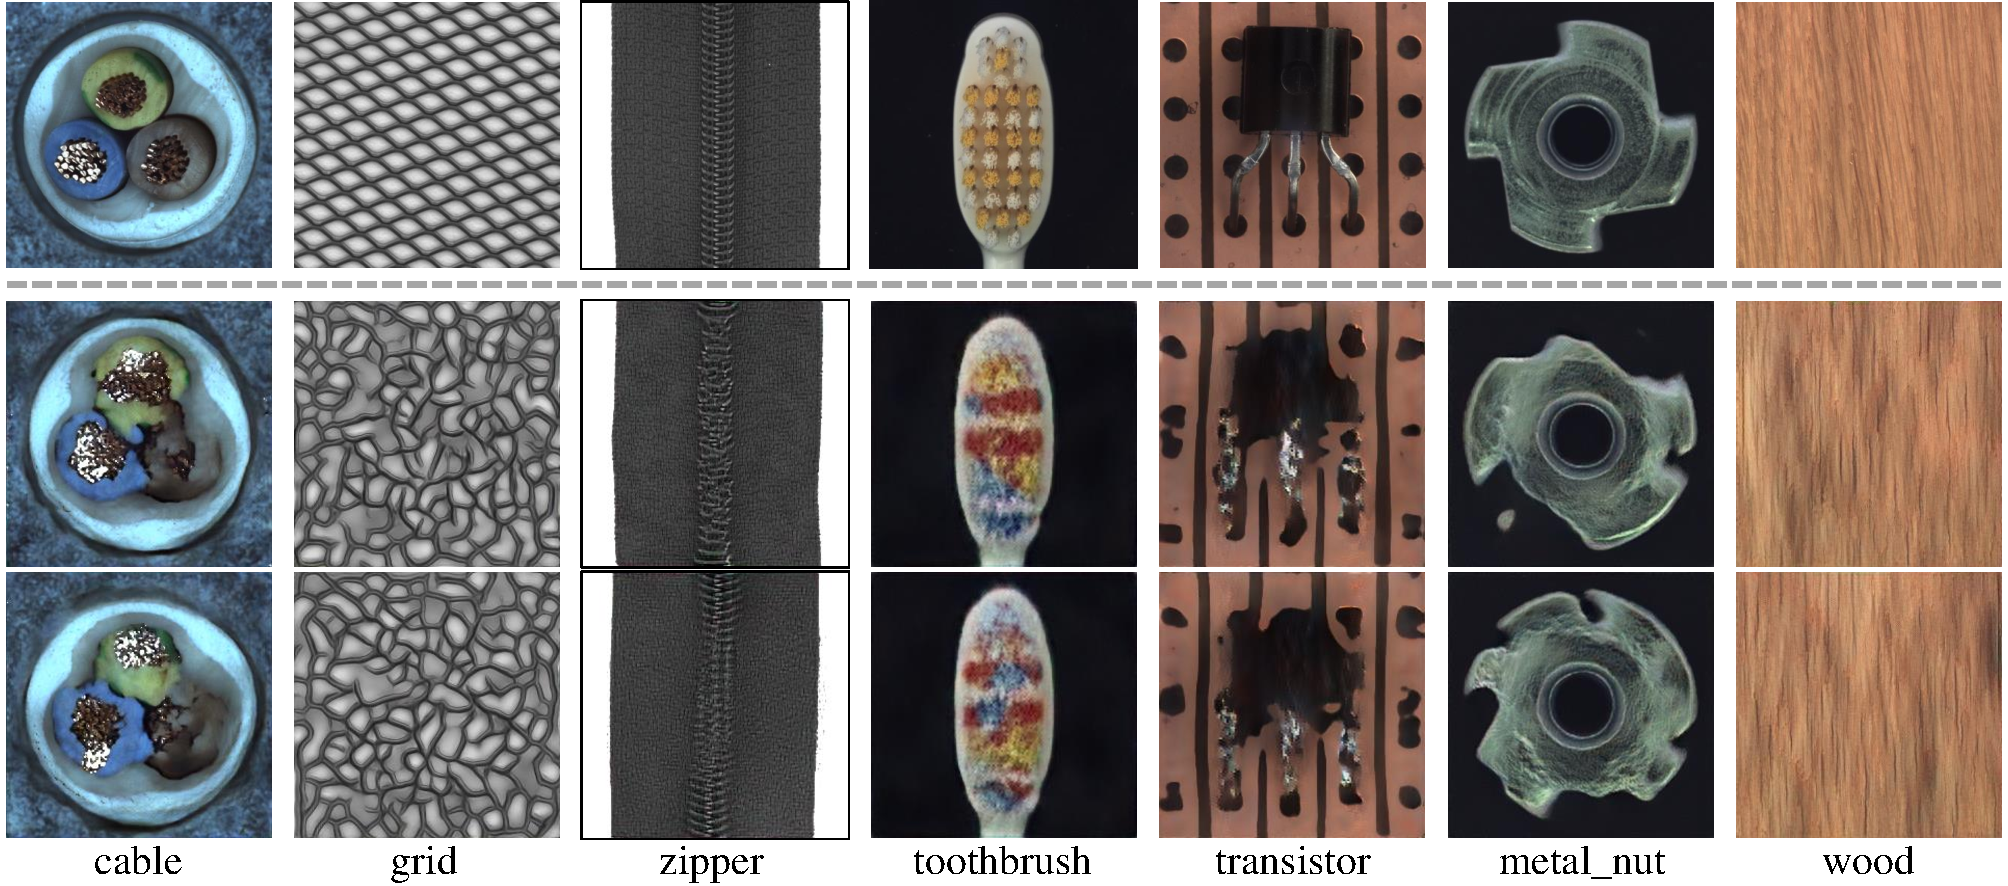
\includegraphics[width=0.7\linewidth]{images/mvtec_generation_results.pdf}
    \caption{Contrastive images generated by level-13 PatchDiff for MVTec AD~\cite{MVTecAD}. } 
    \label{fig: mvtec_generation}
\end{figure*}

\begin{table*}[!h]
    \centering
    % \footnotesize
    % \setlength{\belowcaptionskip}{0.2cm}
    % \setlength{\abovecaptionskip}{0.0cm}
    \renewcommand{\arraystretch}{1.2}
    \resizebox{\textwidth}{!}
    {
\begin{tabular}{cl|c|c|c|c|c|c|c|c}
\toprule
% \multicolumn{2}{c|}{Category} & \makecell[c]{IGD\\\tiny{\citealp{IGD}}} & \makecell[c]{PSVDD\\\tiny{\citealp{PSVDD}}} & \makecell[c]{FCDD\\\tiny{\citealp{FCDD}}} & \makecell[c]{CutPaste\\\tiny{\citealp{CutPaste}}} & \makecell[c]{NSA\\\tiny{\citealp{NSA}}} & \makecell[c]{DRAEM\\\tiny{\citealp{DRAEM}}} & \makecell[c]{DSR\\\tiny{\citealp{DSR}}} & \makecell[c]{GRAD\\\tiny{Ours}} \\ \midrule
\multicolumn{2}{c|}{Category}     & IGD & PSVDD & FCDD & CutPaste &NSA & DRAEM & DSR & GRAD \\ \midrule
\multirow{5}{*}{Texture} 
& carpet & (94.7, 82.8 ) & (92.9, 92.6) & (96.0, - ) & (93.1, 98.3) & (95.5, 95.6) & (95.5,97.0) & (-, \textbf{100.}) & (\textbf{96.5}, 98.2) \\
& grid & (97.7, 97.8 ) & (94.6, 100.) & (91.0, - ) & (\textbf{99.9}, 97.5) & (99.2, 99.9) & (99.7, 99.9) & (-, \textbf{100.}) & (97.2, \textbf{100.}) \\
& leather & (99.5, 95.8) & (90.9, 98.6) & (98.0, - ) & (\textbf{100.}, 99.5) & (99.5, 99.9) & (98.6, \textbf{100.}) & (-, \textbf{100.}) & (98.8, \textbf{100.}) \\
& tile & (78.0, 99.1) & (97.8, 91.4) & (91.0, - ) & (93.4, 90.5) & (\textbf{99.3}, \textbf{100.}) & (99.2, 99.6) & (-, \textbf{100.}) & (95.4, \textbf{100.}) \\
& wood & (89.1, 94.6) & (96.5, 90.8) & (88.0, - ) & (\textbf{98.6}, 95.5) & (90.7, 97.5) & (96.4, \textbf{99.1}) & (-, 96.3) & (87.2, 98.3) \\
\midrule
\multirow{10}{*}{Object} 
& bottle & (92.2, \textbf{100.}) & (98.6, 98.1) & (97.0, - ) & (98.3, 97.6) & (98.3, 97.7) & (\textbf{99.1}, 99.2) & (-, \textbf{100.}) & (96.5, \textbf{100.}) \\
& cable & (84.7, 90.6) & (90.3, 96.8) & (90.0, - ) & (80.6, 90.0) & (96.0, 94.5) & (94.7, 91.8) & (-, 93.8) & (\textbf{98.4}, \textbf{99.3}) \\
& capsule & (\textbf{97.7}, 91.5) & (76.7, 95.8) & (93.0, - ) & (96.2, 97.4) & (97.6, 95.2) & (94.3, \textbf{98.5}) & (-, 98.1) & (97.1, 96.4) \\
& hazelnut & (98.0, 99.7) & (92.0, 97.5) & (95.0, - ) & (97.3, 97.3) & (97.6, 94.7) & (\textbf{99.7}, \textbf{100.}) & (-, 95.6) & (96.6, 98.1) \\
& metal nut & (92.6, 91.3) & (94.0, 98.0) & (94.0, - ) & (99.3, 93.1) & (98.4, 98.7) & (\textbf{99.5}, 98.7) & (-, 98.5) & (93.7, \textbf{100.}) \\
& pill & (97.3, 87.3) & (86.1, 95.1) & (81.0, - ) & (92.4, 95.7) & (\textbf{98.5}, \textbf{99.2}) & (97.6, 98.9) & (-, 97.5) & (98.1, 95.7) \\
& screw & (97.0, 82.5) & (81.3, 95.7) & (86.0, - ) & (86.3, \textbf{96.7}) & (96.5, 90.2) & (97.6, 93.9) & (-, 96.2) & (\textbf{99.2}, 96.0) \\
& toothbrush & (97.7, 99.7) & (\textbf{100.}, 98.1) & (94.0, - ) & (98.3, 98.1) & (94.9, \textbf{100.}) & (98.1, \textbf{100.}) & (-, 99.7) & (98.0, 99.7) \\
& transistor & (84.4, 90.6) & (91.5, 97.0) & (88.0, - ) & (95.5, 93.0) & (88.0, 95.1) & (90.9, 93.1) & (-, 97.8) & (\textbf{97.8}, \textbf{100.}) \\
& zipper & (96.7, 97.0) & (97.9, 95.1) & (92.0, - ) & (\textbf{99.4}, 99.3) & (94.2, 99.8) & (98.9, \textbf{100.}) & (-, \textbf{100.}) & (98.3, 99.7) \\
\midrule
\multicolumn{2}{c|}{Average} & (93.1, 93.4) & (92.5, 93.2 ) & (92.1, 95.7) & (95.2, 96.0) & (96.3, 97.2) & (\textbf{97.3}, 98.0) & (-, 98.2) & (96.8, \textbf{98.7}) \\
\bottomrule
\end{tabular}}
\caption{Anomaly detection performance on MVTec AD dataset~\cite{MVTecAD}. Both pixel-level (left) and image-level (right) AUROC results are shown in each column. The best results are in bold.}
\label{tab: mvtec_main_detail}
\end{table*}

\subsection{Anomaly Detection and Localization}
In the main body, we exclusively present the averaged performance comparison on MVTec AD. In this section, we extend our analysis to provide a detailed result of the anomaly detection and localization performance across each individual sub-dataset within MVTec AD, and display anomaly maps on MVTec AD in Fig.~\ref{fig: main_mvtec_ad_results}. As shown in Table~\ref{tab: mvtec_main_detail}, we compare GRAD to IGD~\cite{IGD}, PSVDD~\cite{PSVDD}, FCDD~\cite{FCDD}, CutPaste~\cite{CutPaste}, NSA~\cite{NSA}, DRAEM~\cite{DRAEM}, and DSR~\cite{DSR}, all of which are independent of pretrained feature extractors. It is easy to find GRAD achieves a strong detection and localization of anomalies.  

\begin{figure*}[!h]
    \centering
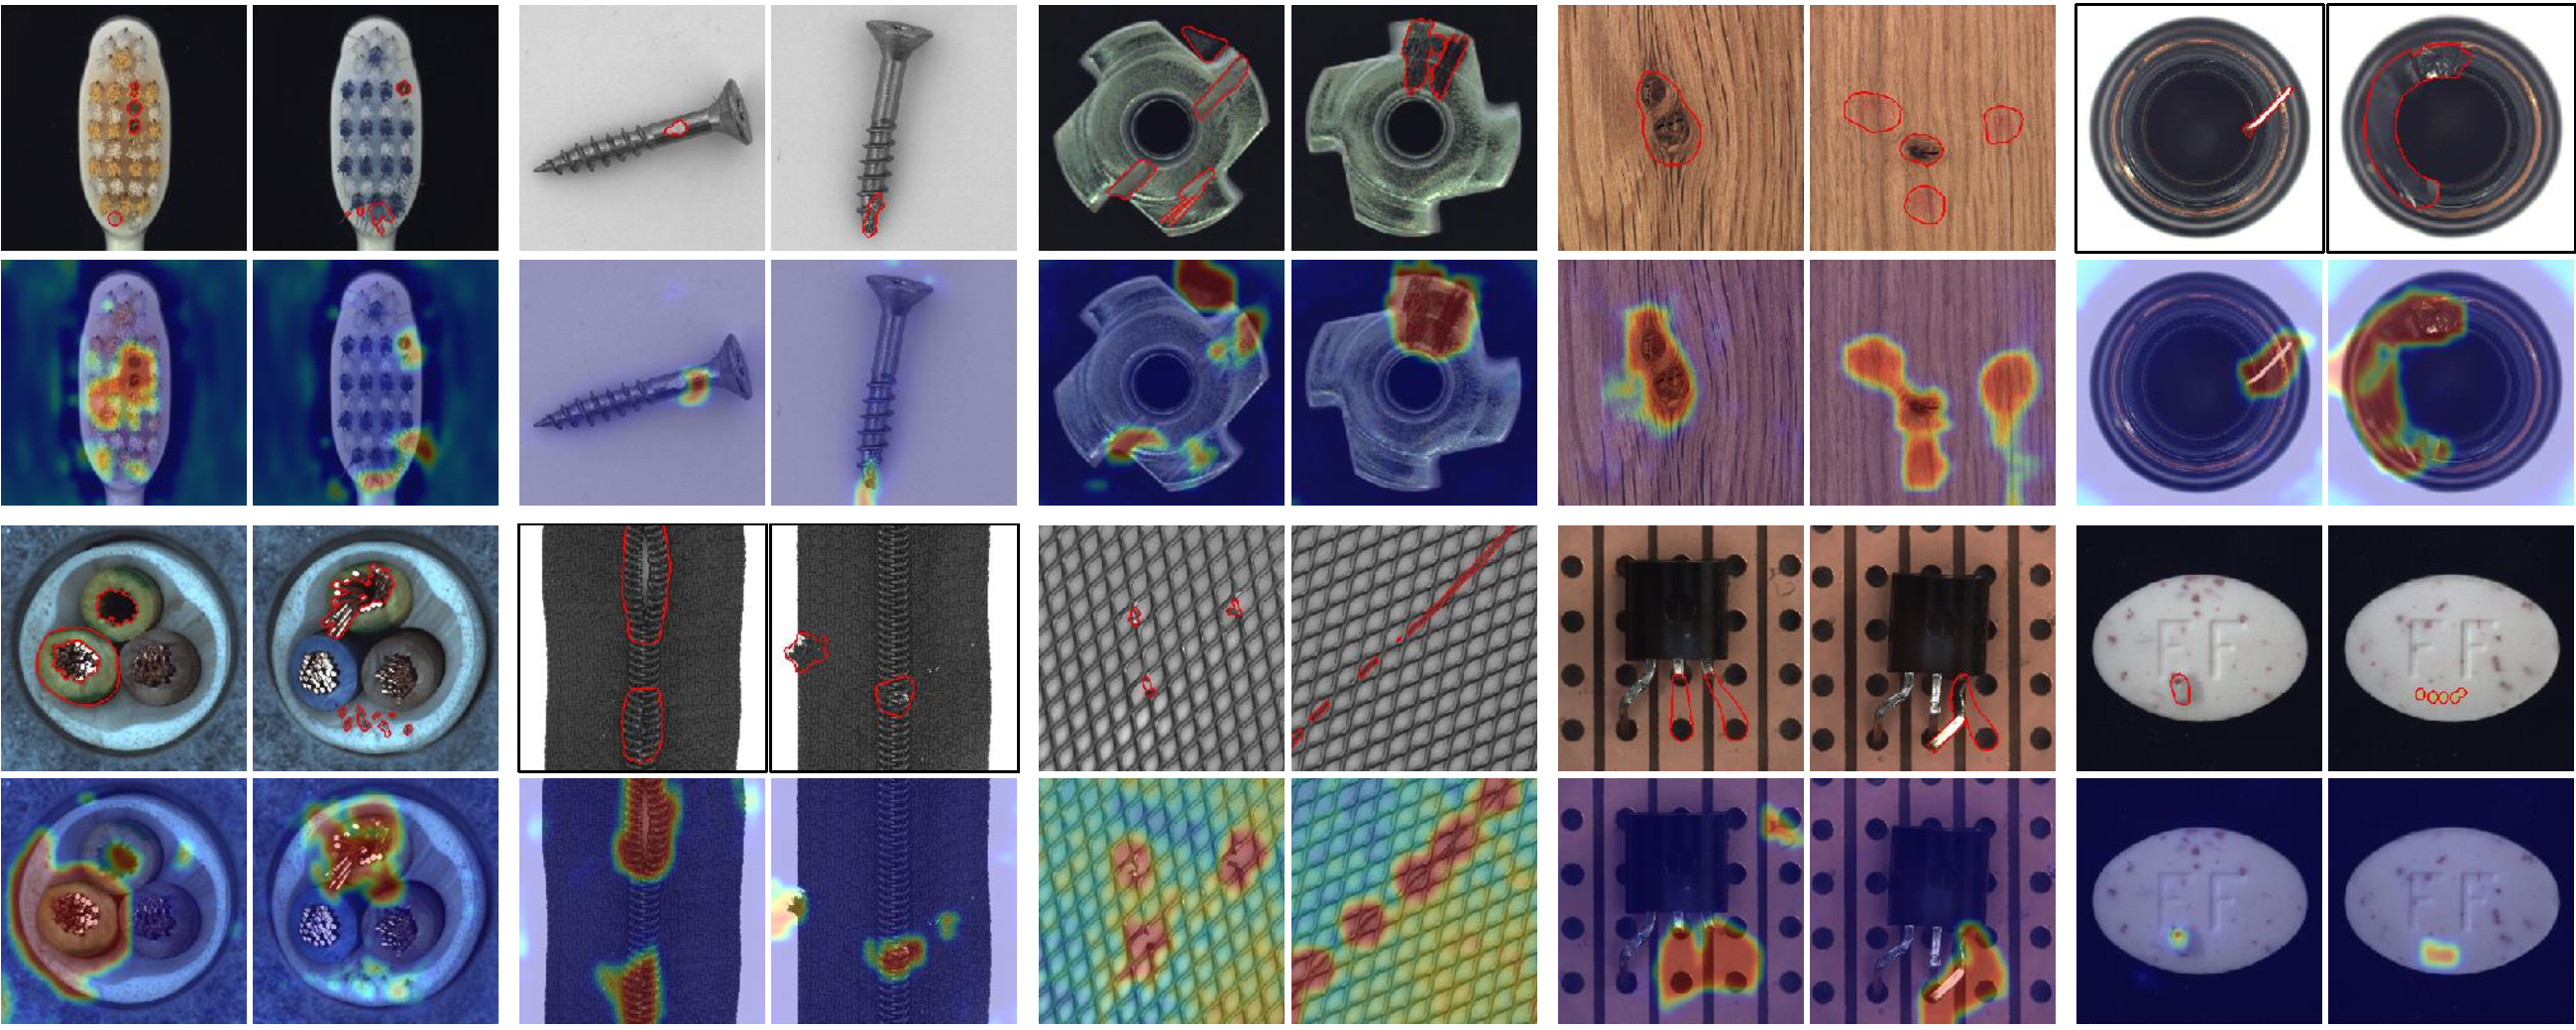
\includegraphics[width=0.9\linewidth]{images/mvtec_results.pdf}
    \caption{Defect localization results of GRAD on MVTec AD~\cite{MVTecAD}. } 
    \label{fig: main_mvtec_ad_results}
    % \vspace{-0.2cm}
\end{figure*}


% In addition, as shown in Table~\ref{tab:ablation_GRad_level}, we conduct an ablations study on selecting levels of patch-level detectors. It is easy to find that when integrating all three different levels of detectors, GRAD can achieve a strong performance for the detection of structural as well as logical anomalies.

% \begin{table}[!htbp]
% \centering
% \footnotesize
% \resizebox{0.3\textwidth}{!}{
% \begin{tabular}{ccc|c}
% \toprule
% \multicolumn{3}{c|}{Level Settings}& Image-level \\
% 136 & 68 & 34  & AUROC\\
% \midrule
% \checkmark &   \ding{55} & \ding{55}   &  85.2   \\
% \ding{55}& \checkmark & \ding{55} & 85.4 \\
% \ding{55}&\ding{55} & \checkmark & 75.1\\
% \checkmark & \checkmark & \ding{55}   &  86.8     \\ %
% \checkmark &   \ding{55} & \checkmark   &  86.4   \\
% \ding{55} & \checkmark & \checkmark  & 86.2 \\
% \checkmark & \checkmark & \checkmark &  \textbf{87.5}  \\
% \bottomrule
% \end{tabular}}
% \caption{Ablation study on detector levels. Detection AUROC results on MVTec LOCO dataset. The best results are in bold.}
% \label{tab:ablation_GRad_level}
% \end{table}



% \bibliography{aaai24}
% \bibliographystyle{aaai24}

% \end{document}


Fugit commodi dicta, vitae fuga ipsa cumque rem vero sequi illum, qui deleniti inventore dolore ut blanditiis fugiat aliquid consectetur magni, deserunt cum soluta numquam odit?Accusantium quisquam voluptas excepturi consequuntur ducimus dolore quidem error quaerat facere, omnis tempora corporis voluptatibus aliquam
\bibliography{aaai22}




\end{document}